\chapter{Problem analysis} \label{chap:problem}

\section*{}

The evaluation for certification is one complex process, and requires many approaches, some acquired knowledge and some experience. To understand the problem and objectives of this dissertation, it is necessary to understand what is CMMI, in particular the SCAMPI method and what is SCRAIM.

\section{CMMI}

To understand better what is CMMI we need to understand what is Capability model.

\subsection{CMM}
A CMM (Capability Maturity Model), including CMMI, is a simplified representation of the world around us. Capability Maturity Models contain essentially elements of effective processes, this elements are based on concepts developed by Crosby, Deming, Juran, and Humphrey.

The SEI (The Carnegie Mellon Software Engineering Institute that is a federally funded research and development center headquartered on the campus of Carnegie Mellon University in Pittsburgh, Pennsylvania, United States) adopted the process management premise, "the quality of a system or product is highly influenced by the quality of the process used to develop it and keep it" and defined CMMs that incorporated this premise.
\begin{figure}[h]
	\begin{center}
		\leavevmode
		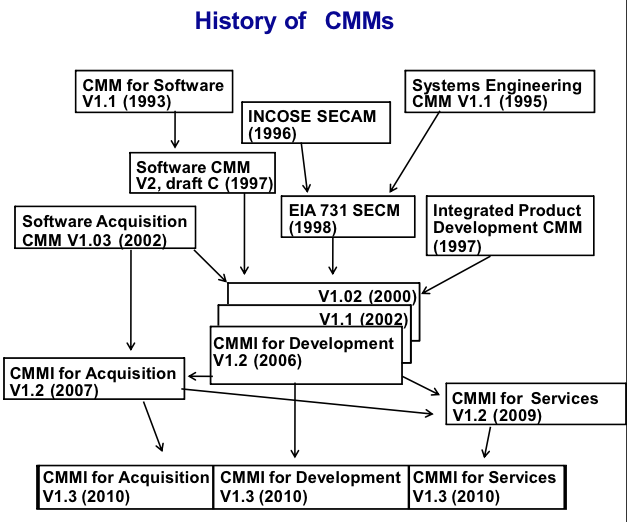
\includegraphics[width=0.86\textwidth]{CMMI_constelations}
		\caption{History of CMMs}
		\label{fig:arch}
	\end{center}
\end{figure}

\subsection{What is CMMI}
CMMI stands for Capability Maturity Model Integration and is a process of improvement training, an appraisal program and a service that is administered and sold by the Carnegie Mellon University, and for some business activities is required and mandatory like many DOD (United States Department of Defense) and U.S. Government contracts, especially in software development.

Carnegie Mellon University says that CMMI can be used to guide an organization, a division and process improvement across projects. The CMMI processes and methodologies can be classified according to maturity levels.

Currently CMMI is on Version 1.3 and is registered in the United States Patent and Trademark Office by Carnegie Mellon University.

\subsection{CMMI models and process areas}
Best practices of CMMI are published in documents called models, each models is addressed to a different area of interest. The current version of CMMI, version 1.3, has three different areas of interest: development, acquisition and services.

These models are produced taking for base the CMMI framework that contains all the goals and practices used to produce the models that are part of CMMI constellations. The CMMI models contain 16 core process areas, they cover basic concepts fundamental to process improvement in any area of interest. 

The material in core process areas it is almost the same for all constellations of CMMI, the rest of the material need to be adjusted to a specific area of interest, so the material wont be the exactly the same.

\subsection{CMMI model framework}
CMMI framework is a basic structure that organizes and groups the CMMI components, elements of the current models, rules, methods for model generations, appraisal methods and training material, contains too process areas that will vary for each one of the CMMI areas that will be used. Process areas are the areas that cover the organization processes.

For the latest version of CMMI for Development (Version 1.3) there are 22 Process Areas, which represents the product aspects and the coverage for the organizational processes.

\subsection{Maturity levels in CMMI for development}
\begin{figure}[h]
	\begin{center}
		\leavevmode
		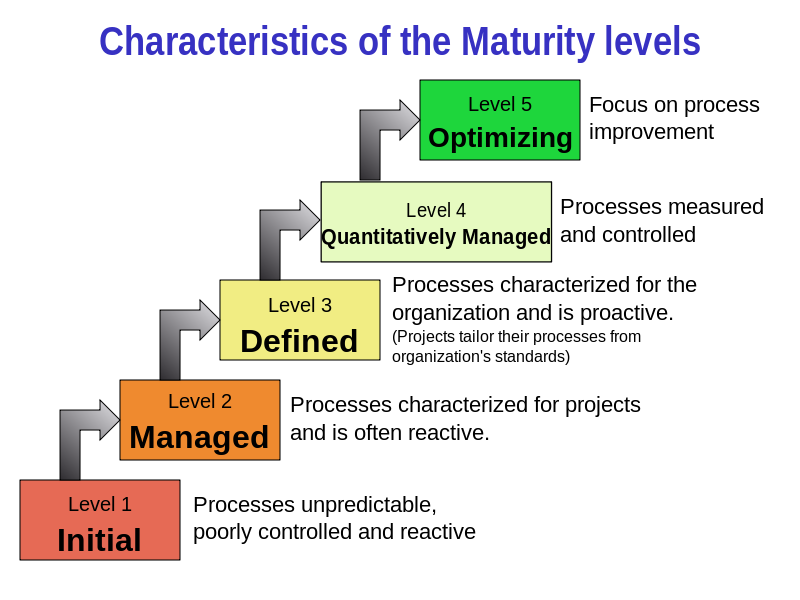
\includegraphics[width=0.86\textwidth]{Maturitylevels}
		\caption{CMMI maturity levels}
		\label{fig:arch}
	\end{center}
\end{figure}
Processes under the CMMI methodology are rated and grouped according levels, called maturity levels. There are five levels of maturity levels defined as: Initial, Managed, Defined, Quantitatively Managed, Optimizing. These maturity levels that are rated are presented and awarded for levels 2 through 5. The following process areas listed show us the maturity levels for CMMI for Development:

\begin{itemize}
	\item Maturity Level 2 - Managed
	\begin{itemize}
		\item CM - Configuration Management
		\item Measurement and Analysis
		\item PMC - Project Monitoring and Control
		\item PP - Project Planning
		\item PPQA - Process and Product Quality Assurance
		\item REQM - Requirements Management
		\item SAM - Supplier Agreement Management

	\end{itemize}
	\item Maturity Level 3 - Defined
	\begin{itemize}
		\item DAR - Decision Analysis and Resolution
		\item IPM - Integrated Project Management
		\item OPD - Organizational Process Definition
		\item OPF - Organizational Process Focus
		\item OT - Organizational Training
		\item PI - Product Integration
		\item RD - Requirements Development
		\item RSKM - Risk Management
		\item TS - Technical Solution
		\item VAL - Validation
		\item VER – Verification	
	\end{itemize}
	\item Maturity Level 4 - Quantitatively Managed
	\begin{itemize}
		\item OPP - Organizational Process Performance
		\item QPM - Quantitative Project Management		
	\end{itemize}
	\item Maturity Level 5 - Optimizing
	\begin{itemize}
	\item CAR - Causal Analysis and Resolution
	\item OPM - Organizational Performance Management
	\end{itemize}
\end{itemize}


\subsection{Appraisal}
Organizations cannot be certified in CMMI, so there is something called appraisal and an organization is appraised.

In an appraisal the organization gets awarded a maturity level from one to five or a capability level achievement profile. As said before many organizations are required to get some kind of recognition and others find value measuring their progress such determine how well the processes adopted by the organization are compared to CMMI best practices, to meet contractual and customers requirements and to know which areas they can improve and appraisals are the right way to do it.

Appraisals using a CMMI model must comply with the requirements set out in the Appraisal Requirements for CMMI (ARC) document. There are three classes of appraisals, A, B and C, all of them compare the processes used in the organization to CMMI processes and best practices, that way is identified improvements to make. From all three classes of appraisals the most formal is class A and it is the only one that can output a level rating.

When an appraisal is done teams use a CMMI model and an ARC document. The results from the teams are used to plan improvements for the organization.

Statistics are made and updated every six months in a maturity profile since the release of CMMI show us that the median times to move from Level 1 to Level 2 is 5 months, from that to Level 3 more 21 months.

\subsection{SCAMPI}
SCAMPI is the abbreviation for Standard CMMI Appraisal Method for Process Improvement and is an appraisal method that meets all the ARC requirements.
In SCAMPI appraisals there are three types of distinct classes: Class A, B and C appraisal methods. The most rigorous method and officially recognized as that is the Class A method, it is the only method that can result in a benchmark quality rating. SCAMPI B and C provide organizations improvements less formal than the class A, however still can identify improvements to be done.

Results SCAMPI appraisal can be published on the CMMI web site of SEI, if the organizations approves this. This appraisal supports the conduct of ISO/IEC 15504, Software Process Improvement and Capability Determination (SPICE), a set of technical standards documents for the computer software development process and related business management functions.

The ARC Class A appraisals is normally conducted by SCAMPI A appraisal. The SCAMPI A Method Definition Document is where its defined rules to ensure the consistency of the appraisal ratings, so the same maturity rated in two companies means they are equal in methodologies and business processes.


\subsubsection{Principals}
As said before the class A appraisal is the only full comprehensive appraisal method that involves an ARC class A method and uses CMMI models as reference models.

This appraisal will allow organizations to gain insight about their capability by identifying the strengths and weaknesses of its current processes, prioritize improvement plans, focus on those improvements, correcting weakness that will generate risks, derive capability rating as a maturity level rating and identify risks relative to capability and maturity determinations.

This appraisal follows this principals:
\begin{itemize}
	\item Start with a process reference model.
	\item Use a defined appraisal method.
	\item Involve senior management as an appraisal sponsor.
	\item Observe strict confidentiality and non-attribution.
	\item Approach the appraisal collaboratively. (When SCAMPI is used for Supplier Selection or Process Monitoring modes, it may not be
	possible to use a collaborative appraisal approach.)
	\item Focus on the sponsors business objectives
\end{itemize}

\subsubsection{Special Terms}
There are some terms to consider with special meaning, Organizational Unit (OU), Organizational Scope, Subgroup, Basic Unit, Support Function, Objective Evidence, Instantiation, Database of Objective Evidence, Practice Characterization.

Organizational Unit is the subject of an appraisal. Can be deployed one or more processes that have a consistent process context, operates in a coherent set of business objectives and is typically part of a larger organization. In a small organization, this unit can be the whole organization.

Basic Unit stands for a set of interrelated and managed resources that delivers products or services to a customer and usually works like planned. The plan is documented and specifies the services or products delivered or implemented, the funds, the future work and the work that is currently being done.

A collection of basic unit and support functions that represent practices used within and organizational unit is the Organizational scope.


A Subgroup is a cluster of basic units that are shared between similar process implementations and a common sampling factor alternatives.



Support Function: An organizational group that provides products and/or services for ax
bounded set of activities needed by other portions of the organization.
Examples of support functions include a configuration management
group or an engineering process group.

Objective Evidence (OE)
Artifacts or affirmations used as indicators of the implementation or
institutionalization of model practices.

Instantiation
The implementation of a model practice used in the appropriate context
within the boundaries of an organizational unit.
another:The implementation of a model practice used in the
appropriate context within the boundaries of an organizational
unit.

\begin{figure}[h]
	\begin{center}
		\leavevmode
		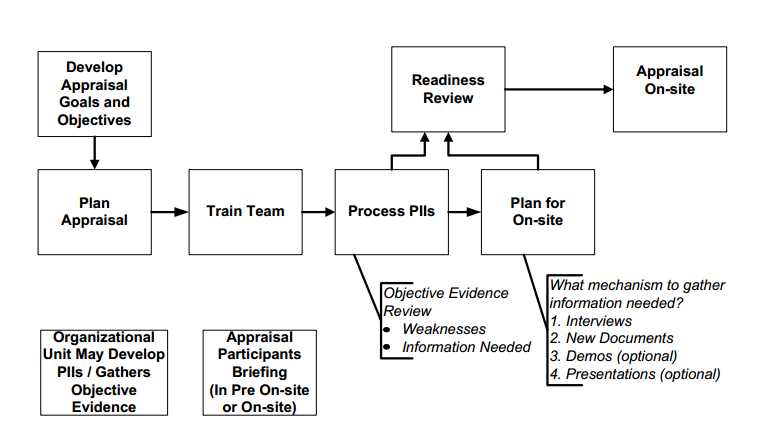
\includegraphics[width=0.86\textwidth]{appraisal_activies}
		\caption{SCAMPI A activities}
		\label{fig:arch}
	\end{center}
\end{figure}


\subsubsection{Appraisal Participants – Roles and Responsibilities}

Objective evidence are “footprints” which are
indicators of the implementation or
institutionalization of model practices. SCAMPI appraisals use objective evidence as
the focus to verify practice implementation.
Verifying practice implementation is the review
of Objective Evidence to determine whether a
practice is implemented within a basic unit,
support function, and/or organization.

Artifacts are
• A tangible form of objective evidence indicative of work being
performed that represents either the primary output of a model
practice or a consequence of implementing a model practice

Examples:
• Example work products listed in CMMI practices
• Target products of an “establish and maintain” specific practice
• Documents, deliverable products, training materials, meeting
minutes, etc.

Affirmation are
• An oral or written statement confirming or supporting
implementation (or lack of implementation) of a model practice
provided by the implementers of the practice, provide via an
interactive forum in which the appraisal team has control over the
interaction.
Examples:
• oral affirmations include interview responses, presentations, and
demonstrations, as long as these presentations and
demonstrations are provided in an interactive setting.
• written affirmations include written statements provided by the
implementers of the practice to the appraisal team via an
interactive forum.


Artifacts
• A tangible form of objective evidence indicative of work being performed that represents either the primary output of a model practice or a consequence of implementing a model practice.
Affirmations
• An oral or written statement confirming or supporting implementation (or lack of implementation) of a model practice provided by the implementers of the practice, via an interactive forum in which the appraisal team has control over the interaction.

For some practices, documents are accepted as artifacts even if they
are not the primary intended result of performing the practice. For
example:
• CM SP1.2 Establish a configuration management system (this
could be represented by a schematic or a description of the
library system from a CM plan)
• PI SP1.2 Establish the product integration environment (this
could be represented by a schematic, a description from an
engineering plan, or a picture)
• GP 2.5 Train people (this could be represented by training
records showing that specific individuals have completed specific
training)

\subsubsection{Practice Characterization (table)}


\subsubsection{Appraisal sponsor - Sponsors appraisal}
- Owns appraisal results
- Signs ADS
Middle managers - From line or staff management positions
- Interviewee and data provider
- *Review preliminary findings
Basic Unit leaders - Leadership responsibilities for a project, service, etc.
- Interviewee and data provider
- *Review preliminary findings
Support Function - Practitioner
- Interviewee and data provider
- Review preliminary findings


\subsubsection{Appraisal Team – Key Roles}

\subsubsection{Team Leader Responsibilities}

\subsubsection{Team Member Responsibilities}

(Why Mini-teams? slide 47)
Mini-Team Responsibilities